%TODO intro

\section{Parsing Vue.js}

\subsection{Assumptions}
It is assumed that the Vue.js code, for which interaction diagrams are going to be generated, compiles and does not contain syntactical errors. No checks are performed in order to verify that. Naturally, logical errors are not an issue.
\subsection{Limitations}
\label{concept:parsing_limits}

In order to be able to generate interaction diagrams, which capture every aspect of Vue.js, the generation must be directly based on an \gls{ast}, which covers every possible syntax, such as \cite{eslint_vue_parser}. 

This thesis only includes the following features of Vue.js:
\begin{itemize}
    \item Event handlers (including anonymous method syntax and method reference syntax)
    \item Any one or two-way binding expressions (\code{v-model}, \code{v-bind}, "moustache", \code{v-if}) excluding \code{v-else}
    \item nested \code{v-for} statements for lists, excluding iterating through properties of an object or iteration with index (property zipped with index)
    \item distinguishing between properties and computed properties
    \item complex object and nested lists models 
    \item methods, including the resolution of arguments, they have been called with (excluding methods called with other methods as arguments)
\end{itemize}

\subsection{AST}

\begin{lstlisting}[style=antrl]
grammar js_simplified;

program: bindings methodDefinitions createdMethod topLevelProperties computedProperties;

topLevelProperties: thisIdentifier*;
methodDefinitions: methodDefinition*; 
createdMethod: methodDefinition;
computedProperties: (thisIdentifier reads writes calls)*;

methodDefinition: thisIdentifier methodArgs reads writes calls;

methodArgs: NAME_IDENTIFIER*;
reads: accesedVariable*;
writes: accesedVariable*;
calls: calledMethod*;

calledMethod: calledMethodIdentifier '(' calledArgs ')';
accesedVariable: identifier;
calledArgs: (calledMethod | accesedVariable)*;

bindings: binding*;
binding: tag accesedVariable | calledMethod BINDING_TYPE;

tag: name tagId loc;
tagId: LINE '_' COLUMN '_' LINE '_' COLUMN;
name: UNICODE | identifier;
loc: start end;
start: LINE COLUMN;
end: LINE COLUMN;

calledMethodIdentifier: THIS id* NAME_IDENTIFIER | id* NAME_IDENTIFIER;

thisIdentifier: THIS identifier;
identifier: NAME_IDENTIFIER id*;
    
id: NUMERIC_INDEX | GENERIC_INDEX | NAME_IDENTIFIER;

//terminals, tokens
LINE: [0-9]+;
COLUMN: [0-9]+;

BINDING_TYPE: 'event' | 'one-way' | 'two-way';
GENERIC_INDEX: 'i' | 'j' | 'k' | 'l' | 'm' | 'n';
THIS: 'this';

NUMERIC_INDEX: [0-9];
NAME_IDENTIFIER:  JS_IDENTIFIER;
JS_IDENTIFIER:  (UNICODE | '$' | '_') (UNICODE | '$' | '_' | [0-9])*;
UNICODE: [\u0000-\uFFFF];
\end{lstlisting}

A Vue.js \gls{spa}, including all the necessary information for \ref{concept:parsing_limits}, can be defined using the above grammar. 

The application consists of \code{bindings} \code{methodDefinitions} a \code{createdMethod}, \code{topLevelProperties} and \code{computedProperties}. 

The \code{topLevelProperties} represent the \code{data} object of the Vue.js \code{script} tag. Each property will be represented flattened, as a list of identifiers and prefixed with \code{this},in order to indicate it belongs to the top level data object. For example \code{problem:\{a:0, b:0\}} will be represented as follows:

\begin{figure}[H]
    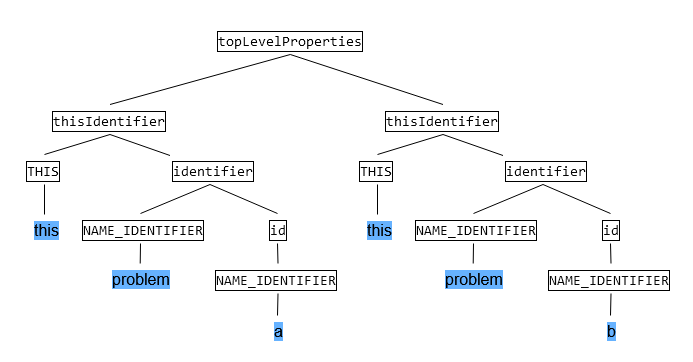
\includegraphics[width=0.8\textwidth]{images/ast_top_level.png}
     \caption{\gls{ast} for top-level example }
     \label{fig:ast_top_level}
\end{figure}

Bindings can be obtained from the Vue.js \code{template}.

Each binding consists of an HTML tag, an a list of binding sources for that tag - pairs of variable or method call and a binding type. The binding type represents the type of the binding - either event, one-way or two-way. Two-way bindings are only valid with properties, whereas for events and one-way bindings, both method calls and properties are possible, since in Vue.js a binding source could be an expressions defined as an inline anonymous functions (
    \code{<div v-if=\"value === true\"/>}
). The binding sources are a list, since a tag could have multiple different bound properties, or a bound expression. The information about how exactly the properties are bound, if it is the same type of binding, is discarded.

Method calls include the parameters they have been called with - other methods or just variables. It is also possible to call methods with binary expressions - those are represented as a special method, which takes 2 parameters - the left and right side operators of the binary expression. Expressions with multiple terms can be represented as multiple binary expressions. This representation loses information such as the order of operations, but since we are only interested in which properties are being accessed, this loss does not pose an issue.

A special case is accessing lists. For example \code{<div v-bind="problems[0].a"/>} would result in the following:

\begin{figure}[H]
    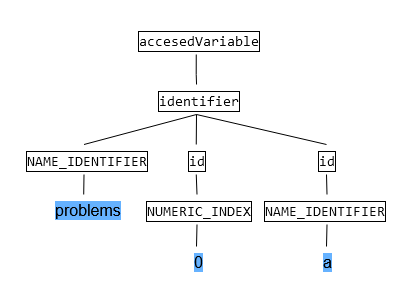
\includegraphics[width=0.8\textwidth]{images/ast_problems_0_a.png}
     \caption{\gls{ast} for example }
     \label{fig:ast_list_simple}
\end{figure}


\code{v-for} statements, are substituted:
\begin{lstlisting}[style=html]
<ul>
  <li v-for="subject in subjects" :key="subject.id">
    {{ subject.problems[0] }}
  </li>
</ul>
\end{lstlisting}
results in
\begin{lstlisting}[style=html]
subjects[i].problems[0]
\end{lstlisting}
which in term produces the following AST:

\begin{figure}[H]
    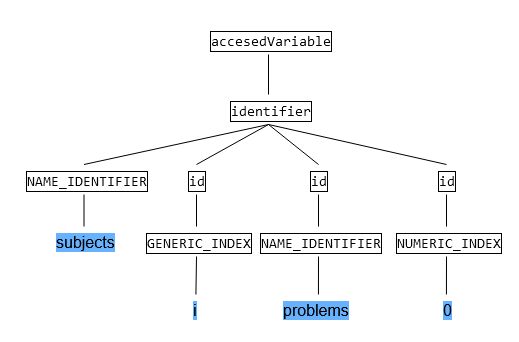
\includegraphics[width=0.8\textwidth]{images/ast_numeric_generic.png}
     \caption{\gls{ast} for example }
     \label{fig:ast_list_complex}
\end{figure}

Nested lists are also possible and would result in multiple generic indices being added.

Each tag includes its location in the source code (starting and ending line and column), which can also be used as an identifier. Tags also have humanly readable names, which are either equal to the the text of the tag, if it exists, or to the identifier of the first binding. 

\code{methodDefinitions} include all methods definitions from the \code{method} object of the \code{view-model}. Each method definition consists of the following
\begin{itemize}
    \item identifier - an identifier, equal to \code{this} followed by the name of the method
    \item arguments - names of arguments, each of which is a simple name identifiers
    \item reads - variable it reads from
    \item writes - varaibles it writes to
    \item calls - method calls, including arguments, same as for bindings 
\end{itemize}

\code{computedProperties} are similar to \code{methodDefinitions} with the exception that they do not have arguments. Albeit bad practise, it is still possible for computed properties to have side effects and therefore it was decided to model them as methods.

%TODO explain compound etc graph
\section{Interaction Diagram Generation}
Interaction diagrams can be generated from the simplfied Vue.js \gls{ast} in the following way.
For each binding (tag, binding sources tuple) in bindings $(t,S) \in bindings$ :

for each binding source $s \in S$
if it is an accesedVariable $v$
check if it is a computed property by looking up the \code{computedProperties}. If true, treat it as a method, which will be explained below. If false, check if it is a property, by checking if there is a top level property in $topLevelPropertiers$, which starts with the same identifier (ignoring the \code{this} prefix).
If true, prefix $this$ and create a node for each $id$ in $identifier$. Create a \gls{guid} for each node, by starting from \code{this} and in sequence iterating over each $id$ in $identifier$ concatenate its $id$ with the $id$ of the node before it and also set it as its parent. Connect those nodes  with unidrectional edges starting from \code{this} and label each edge \textit{data}. Assign a label to each node, equal to its $id$ if it is a \code{NAME_Identifier}, or else to the name of the previous node including the name of the current one in square brackets. % TODO if non exist create
%TODO also include types in text info
\begin{figure}[H]
    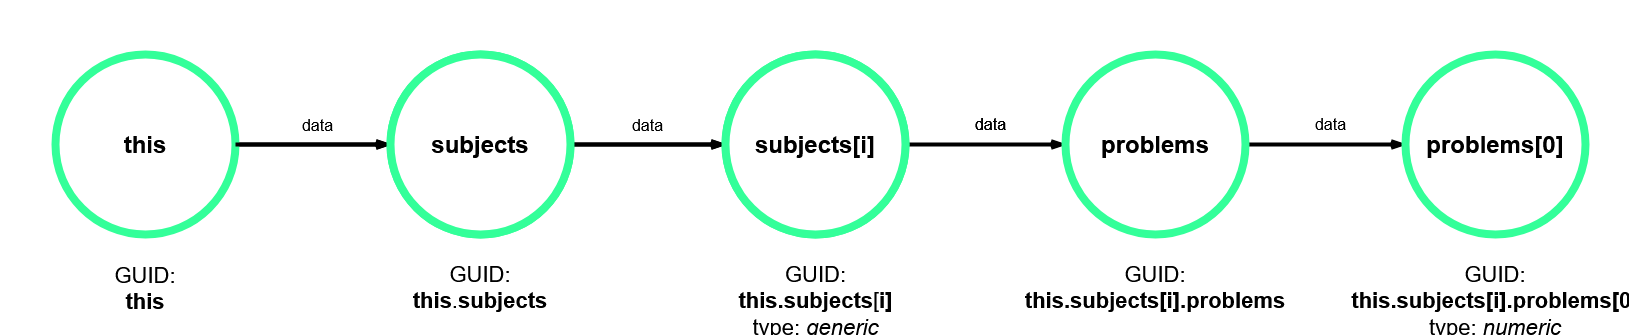
\includegraphics[width=0.8\textwidth]{images/graph_numeric_generic.png}
     \caption{Nodes created for identifiers of \ref{fig:ast_list_complex} }
     \label{fig:ast_list_complex_nodes}
\end{figure}

If the binding source $s$ is a \code{calledMethod}, check if it exists in $methodDefinitions$ by excluding the \code{this} prefix. If true, prefix it with \code{this} and create a node for it. Replace each of it's arguments, which cannot be found in \code{topLevelProperties} or \code{computedProperties} by a fixed word such als $OTHER$ or $*$, join them with $,$ and surround them with brackets. Concatenate it with the name of the method to form the \gls{guid} of the method. Remove \code{this} identifiers from the method name and arguments and and set it as its label.

The node for the method itself is now completed, the next step is to create nodes for it's the properties it $reads$ and $writes$ and for other methods it $calls$, if they do not yet exist based on its $methodDefinition$. The first step is to substituted the method definition arugments with the called arguments and update all $reads$, $writes$ and $calls$ referencing them. Now $reads$, $writes$ and $calls$ which do not start with \code{this} can be removed since they are not properties. After this is done, create a node for each property in $reads$ and $writes$ in the same way as described above. 
For each property in $writes$ add an edge with the property as the source and the current method as the sink. For each property in $calls$ add an edge with current method as the source as the property as the sink.

For each method in $calls$, which does not yet exist in the graph, recursively repeat the above process and add and edge from the current method to it labelled $calls$. 


If any nodes were created in the previos steps, create a node for the tag $t$ with a \gls{guid} $tagId$ and label $name$. Based on the binding type create edges to connect $t$ and each of the nodes.
If the binding type is an event binding, create an 
%todo introduce n for nodes?
edge with source $t$ and sink \textit{node} and label it $event$. 
If the binding type is one-way, create an edge with source \textit{node} and sink $t$.
If the binding type is two-way, create an edge

with source $t$ and sink \textit{node} and label it $event$ and a second edge with source \textit{node} and sink $t$. In essence two-way bindings create the same edges as a combination between one-way and event bindings.

%todo can cause conflicts? no can't cause 'this.method
For the initial method - $createdMethod$ create a node with \gls{guid} and name equal to \textit{created}. Resolve its $reads$, $writes$ and $calls$ in the same maner as methods, described in the previos section.
%Example of all edge types simple

%based on ids connections

%TODO generic/numeric thing of adding more node relations

% TODO comment on how based on "if exists create"
% dynamic, only tohse that icluded left\
% TODO this.x.method assumes mutation of X  
Due to dynamic nature\dots
\section{Scenario Generation}

In order to generated scenarios in Gherkin, interactions can be sliced in a similar manner as described by \textcite{zhang2019scenario} and summarized in \ref{intro:zhang_interaction_diagrams}.

Let $N$ denote the set of all nodes in the graph and $E$ denote all edges in the graph. Let $n \in N$, $m \in N$ be any two nodes in the graph and let $(n, m) \in E $ represent an edge from $n$ to $m$. Let $type(n)$ be a function, that returns the type of a node and $label(n, m)$ be a function that returns the label of the edge from $n$ to $m$. Let $E_{out}(n)$ be a function, which returns all outgoing edges of $n$.
Let $E_{in}(n)$ be a function, which returns all incoming edges to $n$.

Let $N_I$ denote all nodes, that the user can interact with. A node $n \in N$ is also in $N_I$ if $\exists e \in E_{out}(n)$ where $label(e) = event$. Let $N_H$ denone all html tag nodes. a node $n \in N$ is also in $N_H$ if $type(n) = tag$. 
Given a node $n_H \in N_H \cup {created}$, a node $m_H \in N_H$ reacts to $n$ iff
\begin{enumerate}
    \item $\exists n_0,n_1,n_2, \ldots,n_k \in N, n_0=n_H,n_k=m_H$ such that for each $0 \leq i < k  $ $(n_i,n_{i+1}) \in E$, and $label((n_i,n_{i+1}))\neq event$ and if $label(n_i,n_{i+1}) \neq calls$ $\forall n_{i+1_{in}} E_{in}(n_{i+1})$ $label(n_{i+1_{in}}) \neq event$ 
\end{enumerate}

Analogous to \cite{zhang2019scenario} let $l(n)$ denotes all nodes, that react to $n$. A sequence of user interactions, starting with the initial function is refered to as a \textit{scenario} $A=(a_0,a_1,\ldots, a_n)$ where $a_0=created$ and $\forall0 < k \leq n, a_k \in N_I$. 

Define the HTML tags, to which a scenario reacts, to be equal to the tags to which the last tag in the scenario reacts 
- $l(A)=l(a_n)$. 


The set of scenarios is generated by starting with the initial scenario, containing only the initial function $S_0 = \{(created)\}$. It is then prolonged by all tags $n \in N_I$, representing that the user can click anywhere resulting in $N_I$ scenarios of length 2. Scenarios of length 3 are generated by taking the previous ones of length 2 $S_2$ and for each scenario $S in S_2$ generate up to $N_I$ new scenarios by prolonging $S$ with $n | n \in l(S) \cap N_I$
%TODO his def is better.
This is repeated up to $k$ times, where $k$ is a constant set by the user. Then each set is collapsed(%TODO how
) and later only unique interaction are generated.

and prolonging it iteratively by each widget, where the user can take an action.

Gherkin scenarios templated can then be obtained by the following tempalte:
Scenario - $n_0,n_1 \ldots n_k$
Given - $n_0, n_1 \ldots n_{k-1}$
When - $n_k$
Then - $l(n_k)$



%TODO displaying objects, bonus che se vijda tochno koe property se updateva 


%TODO in assumptions no nested lists

%TODO actually also top level, either remove from code or here descrp



% FAZIT
% TODO assumes reads, would have been better treat as anonymous method